\chapter{Особливості використання активного ультразвуку}
Значна частина представлених у дисертаційній роботі результатів пов'язана з дослідженням ефектів, які відбуваються в напівпровідникових структурах внаслідок
поширення в них акустичних хвиль (АХ) мегагерцевого діапазону.
У зв'язку з тим, що використання ультразвуку (УЗ), на жаль, ще не є стандартним способом впливу на напівпровідникові кристали,
у цьому розділі представлено узагальнена  інформація щодо відповідних експериментальних методик.

Зокрема, представлені описи процедур ультразвукової обробки (УЗО) та ультразвукового навантаження (УЗН).
Відмінності у використанні цих термінів пов'язані з оборотністю АІ процесів.
Так, в першому випадку (УЗО), внаслідок поширення пружних хвиль відбуваються незворотні (залишкові) зміни властивостей напівпровідникових структур.
Тоді як в другому випадку (УЗН), ефекти є оборотніми (динамічними), зміни електрофізичних параметрів спостерігаються лише за умов поширення АХ;
після припинення дії УЗ параметри поступово повертаються до своїх вихідних (до початку УЗН) значень.



\section{Методика вивчення ультразвукового впливу}
%В роботі наведено результати досліджень акустоіндукованих (АІ) ефектів в кремнієвих бар'єрних структурах, описаних в розділах \ref{MSSi} та \ref{SSC}.
%Це ефекти полягають у зміні електрофізичних параметрів структур під час поширення в них пружних коливань, тобто під час ультразвукового навантаження (УЗН).
%Ефекти є оборотніми (динамічними), після припинення поширення акустичних хвиль (АХ) параметри поступово повертаються до своїх вихідних (до початку УЗН) значень.
%
Для збудження УЗ у досліджуваних структурах використовувалися п'єзоелектричні перетворювачі,
виготовлені з пластин ніобату літію (LiNbO$_3$) з металізацією обох граней шляхом вакуумного напилення алюмінію.
Для збудження повздовжніх та поперечних акустичних хвиль використовувалися пластини зі зрізом $(Y\!+\!36^\circ)$ та , відповідно.

З літератури \cite{Ostapenko1995,Davletova2008,Davletova2009,Pashaev2014r} відомо, що АХ з частотою, що знаходиться в діапазоні $1\div30$~МГц, здатні впливати на стан дефектів у кремнії.
Саме такий частотний діапазон був використаний у представлених дослідженнях.
В експериментах проводилось збудження УЗ з частотою $f_\mathtt{US}$, яка знаходилась поблизу першої або третьої гармоніки товщинного резонансу пластинки.
Безпосереднє значення $f_\mathtt{US}$, при якому введення пружних коливань у зразок відбувається найбільш ефективно, визначалось стандартним методом за максимальною амплітудою коливань краплі води (або вакуумного масла), розміщеної на поверхні перетворювача, при прикладанні до його граней змінної напруги.

Попередні дослідження різних авторів \cite{Davletova2008,Davletova2009,Pashaev2014r,Vlasov2009r} показали, що використання УЗ з інтенсивністю $W_\mathtt{US}\geq3$~Вт/см$^2$ спричинює необоротні (залишкові) зміни властивостей кремнієвих структур, які пов'язані з відпалом радіаційних дефектів, формуванням нових дефектів або переміщенням вже існуючих, на відстані, що значно перевищують міжатомну відстань.
Так як метою частини роботи було дослідження саме оборотних АІ ефектів, то переважна більшість УЗН проводилось при $W_\mathtt{US} \leq 1,5$~Вт/см$^2$.
Детальніше процедура оцінки $W_\mathtt{US}$ та інших параметрів УЗ впливу наведена у розділі \ref{subLowT}.

Для того, щоб під час УЗН позбавитися впливу п'єзоелектричного поля, яке супроводжує механічні коливання пластини LiNbO$_3$,  як на параметри напівпровідникових структур, так і на процес вимірювання електрофізичних параметрів,
перетворювач екранувався.
Як наслідок, можна стверджувати, що виявлені під час УЗН ефекти визначаються лише знакозмінною деформацією.

Схеми навантаження зразка, які використовувалися в роботі, наведено на Рис.~\ref{figUSL}.
Наявність чи відсутність діелектричного прошарку визначалась особливостями вимірювання ВАХ.
Використання буфера дозволяло найефективніше мінімізувати вплив п'єзоперетворювача на процеси у напівпровіднику:
металевий буфер виконував роль як електричного, так і температурного екрану.
Тип схеми УЗН, яка використовувалася в тих чи інших дослідах, зазначено на початку відповідного розділу.

\begin{figure}
\center
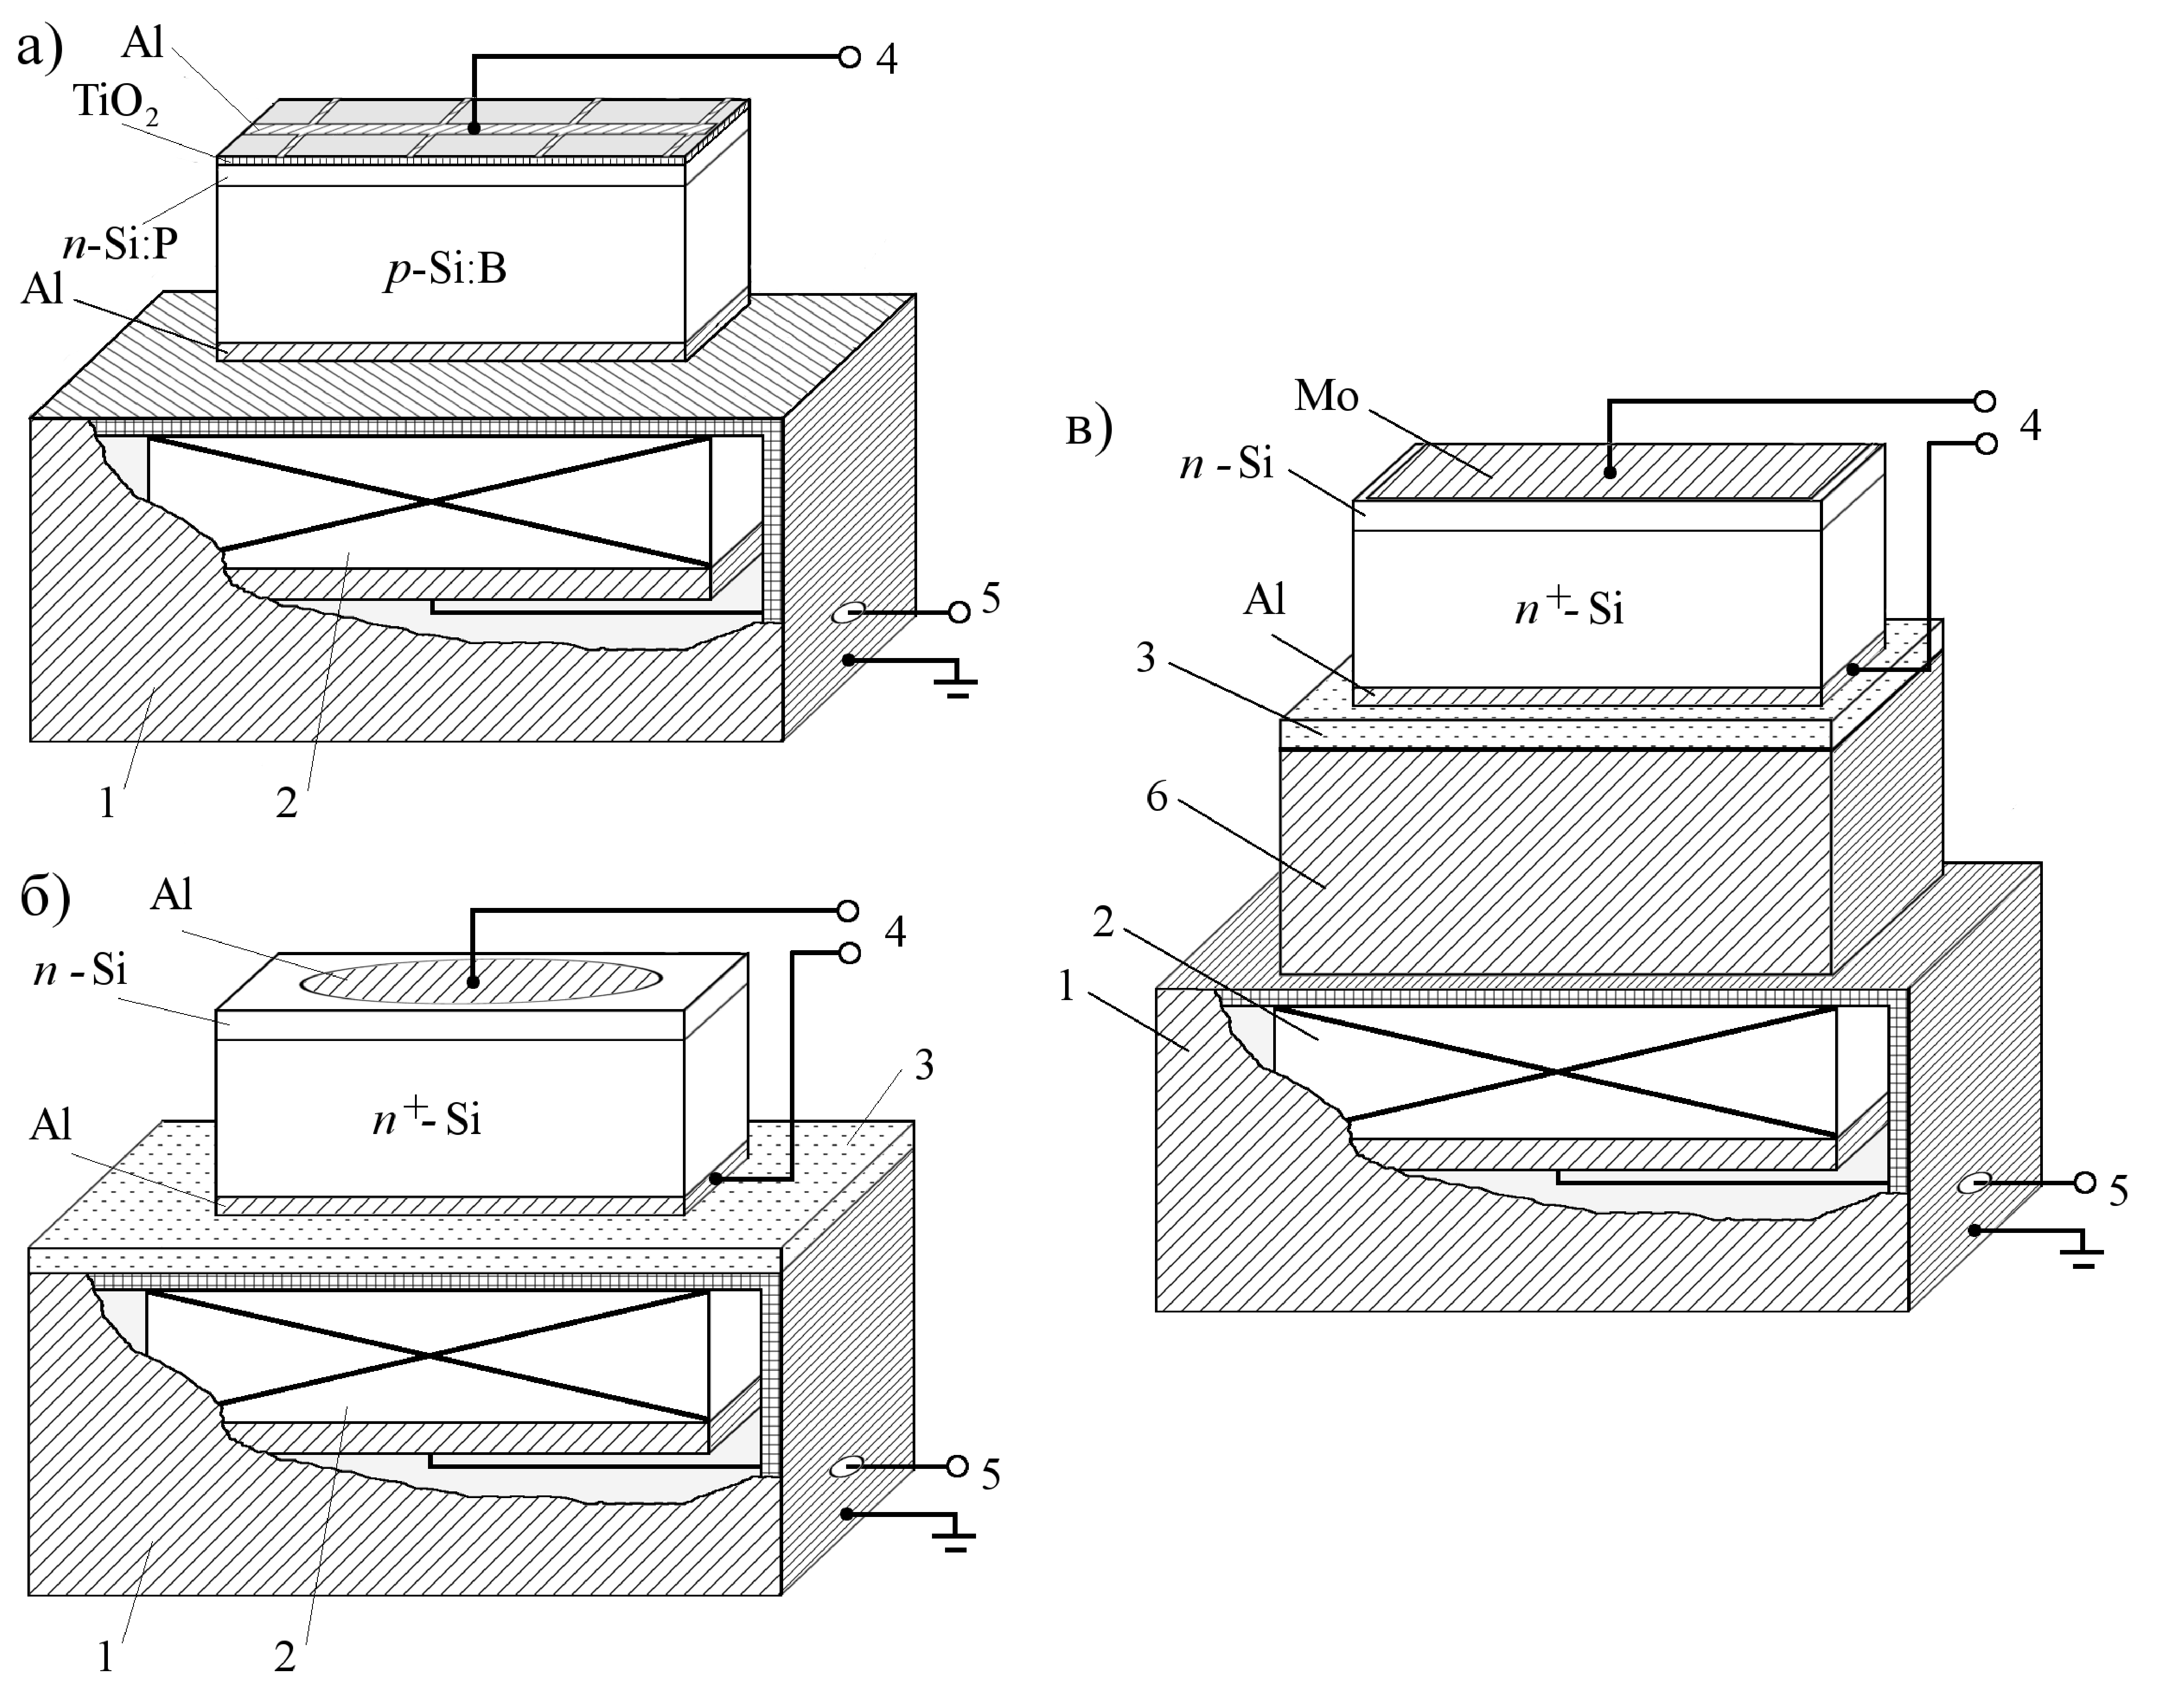
\includegraphics[width=1.0\textwidth]{USL}%
\caption{\label{figUSL}
Використані схеми УЗН.
1 --  екран (алюмінієва фольга, товщина 0,012 мм);
2 --- п'єзоелектричний перетворювач (LiNbO$_3$);
3 --- діелектричний прошарок (слюда, товщина 0,03 мм);
4 --- контакти для вимірювання ВАХ;
5 --- контакти для збудження УЗ;
6 --- буфер (циліндр Al з високим ступенем паралельності граней, довжина 2~см)
}
\end{figure}

Структури, в яких проводилися дослідження ефектів УЗН, містили енергетичний бар'єр, пов'язаний з наявністю контакту МН або p--n переходу і розміщений поблизу однієї з поверхонь зразка.
Введення УЗ відбувалось з боку грані, протилежної до місця розташування бар'єру.
Тобто, напрям поширення АХ перпендикулярний площині бар'єру і співпадає з напрямом струму, який виникає під час прикладення до структури електричної напруги (або при освітленні, якщо об'єктом дослідження є сонячний елемент).
При цьому, при використанні повздовжніх хвиль вимушені зміщення атомів відбуваються у тому самому напрямі, тоді як для поперечних хвиль коливання частинок спрямовані перпендикулярно до електричного струму у площині бар'єру.


Для створення акустичного контакту при різних УЗН використовувалися вакуумне масло, клей БФ6, піцеїн.
Зауважимо, що у випадку низькотемпературного (при $T<230$~К) УЗН процес збудження АХ був утруднений через те, що
рідкі акустичні склейки на кшталт вакуумного масла кристалізувалися і переставали виконувати свою функцію.
В той же час, контакт створений при кімнатній температурі за допомогою жорсткої склейки (піцеїн або БФ6),
руйнувався при охолодженні внаслідок різниці коефіцієнтів теплового розширення.
В роботі проведення низькотемпературних УЗН при використанні повздовжніх хвиль здійснювалось за допомогою свіжого (до 5~год після нанесення) контакту з клею БФ6, який ще не висох.
Наявність акустичного контакту контролювалася за виглядом залежності повного опору перетворювача від частоти (АЧХ, амплітудно--частотної характеристики).
Зокрема, при використанні схеми, зображеної на Рис.~\ref{figUSL},в, за наявності акустичного контакту на АЧХ з'являвся ряд максимумів, пов'язаних з відбиванням хвиль від граней буфера.


Раніше показано \cite{Ostapenko1995,YOlikhTPL2011,Ostrovskii2001}, що характерний час зміни властивостей кремнієвих структур під дією УЗ не перевищує $2\cdot10^3$~c.
Для того, щоб дочекатися закінчення всіх перехідних АІ процесів, використовувалася наступна експериментально процедура.
УЗН починалась при кімнатній температурі.
Після цього зразки перебували не менше 60~хв за умов поширення в них пружних коливань і лише після цього, не припиняючи дії УЗ, починалось вимірювання електрофізичних параметрів та/або процеси нагріву або охолодження.

Відомо, що під час навантаження п'єзоперетворювач нагрівається.
Температура кремнієвих структур контролювалася диференційною термопарою мідь--константан.
В роботі проводилось порівняння значень параметрів, отриманих за однакових температур в умовах УЗН зразків та без нього.
Це дозволяло виокремити АІ зміни характеристик напівпровідникових структур, від змін, пов'язаних з їх розігрівом під час УЗН.
Для оцінки величини впливу УЗ на певний параметр $P$ (яким могла бути напруга холостого ходу, фактор неідеальності, величина зворотного струму тощо),
використовувалися його абсолютні
 \begin{equation}
 \label{eqAbsDelta}
\Delta P=P_{in}-P_\mathtt{US}
 \end{equation}
чи відносні зміни
 \begin{equation}
 \label{eqEpsDelta}
\varepsilon_P=\frac{P_{in}-P_\mathtt{US}}{P_{in}},
 \end{equation}
де нижні індекси <<$\mathtt{US}$>> та <<$in$>> вказують на те, що відповідне значення параметра було отримане при однаковій температурі за умов УЗН та без нього, відповідно.

Таким чином, основними параметрами УЗН є $f_\mathtt{US}$, тип збуджених хвиль, $W_\mathtt{US}$ та температура зразка під час поширення АХ.
Параметри УЗН, які використовувалася в тих чи інших дослідах, зазначено на початку відповідного розділу.

При УЗО процеси впливу АХ та вимірювання параметрів були розділені в часу і тому нагальної необхідності екранування п'єзоелектричних полів не було.
Як наслідок, експериментальна схема простіша, п'єзоперетворювач безпосередньо акустично контактував з досліджуваною структурою.


\section{Оцінка параметрів акустичного впливу\label{subLowT}}
Для оцінки інтенсивності АХ введеної, наприклад, у кремнієву структуру використовувалася формула плоского п’єзоперетворювача \cite{WusBook}:
 \begin{equation}
 \label{eqWus}
 W_\mathtt{US}=4K_\mathtt{LNO}^2C_\mathtt{LNO}f_r\frac{\rho_\mathtt{LNO}\,\upsilon_\mathtt{LNO}}{\rho_\mathtt{Si}\,\upsilon_\mathtt{Si}}\frac{V_\mathtt{RF}^2}{A_\mathtt{LNO}M_0},
 \end{equation}
де
$K_\mathtt{LNO}$ --- коефіцієнт електромеханічного зв'язку,
$C_\mathtt{LNO}$ та $A_\mathtt{LNO}$ --- статична ємність закріпленого перетворювача та його площа, відповідно;
для використаних в роботі перетворювачів ємність складала $(1\div3)\cdot10^{-10}$~Ф залежно від площі та товщини;
$f_r$ --- резонансна частота;
$\rho_\mathtt{LNO}$ та $\rho_\mathtt{Si}$ --- густина LiNbO$_3$ та кремнію, відповідно;
$\upsilon_\mathtt{LNO}$ та $\upsilon_\mathtt{Si}$ --- швидкості поширення звуку в ніобаті літію та Si, відповідно;
$V_\mathtt{RF}$ --- амплітуда високочастотної напруги, прикладеної до перетворювача,
а коефіцієнт $M_0$ розраховується за допомогою співвідношення
 \begin{equation}
 \label{eqM0}
 M_0=\frac{\left[\cos\left(\pi\frac{f_\mathtt{US}}{f_r}\right)\right]^2+\left[\frac{\rho_\mathtt{LNO}\,\upsilon_\mathtt{LNO}}{\rho_\mathtt{Si}\,\upsilon_\mathtt{Si}}\sin\left(\pi\frac{f_\mathtt{US}}{f_r}\right)\right]^2}
 {\left[\sin\left(\frac{\pi}{2}\frac{f_\mathtt{US}}{f_r}\right)\right]^4}.
 \end{equation}
При цьому при поширенні АХ має місце відносна деформація
 \begin{equation}
 \label{eqDefUS}
 \xi_{\mathtt{US}}=\sqrt{\frac{2W_\mathtt{US}}{\rho_\mathtt{Si}\,\upsilon_\mathtt{Si}^3}},
 \end{equation}
а амплітуда зміщень атомів
 \begin{equation}
 \label{eqAmpUS}
 u_{\mathtt{US}}=\sqrt{\frac{W_\mathtt{US}}{2\,\pi^2\,f_\mathtt{US}^2\,\rho_\mathtt{Si}\,\upsilon_\mathtt{Si}}}.
 \end{equation}

Значення резонансної частоти перетворювачів визначалось за допомогою приладу для дослідження АЧХ Х1--38.
Параметри, які використовувалися при розрахунках, наведено в Таблиці~\ref{tabLNO}.


\begin{table}
\caption{\label{tabLNO}Деякі параметри ніобату літію та кремнію при кімнатній температурі \cite{WusBook,ShackBook}.
}
%\begin{tabular}{|l|l|c|}
%\begin{tabularx}{\textwidth}{|>{\raggedright\arraybackslash}X|>{\centering\arraybackslash}X|>{\centering\arraybackslash}X|}
\begin{tabularx}{\textwidth}{|l|>{\centering\arraybackslash}X|>{\centering\arraybackslash}X|}
\hline
$K_\mathtt{LNO}^2$&зріз $(Y\!+\!36^\circ)$&0,24\\
\cline{2-3}
&зріз &0,46\\
\hline
$\upsilon_\mathtt{LNO}$,&повздовжні хвилі&7340\\
\cline{2-3}
м/с&поперечні хвилі&4560\\
\hline
$\upsilon_\mathtt{Si}$,&повздовжні хвилі&8430\\
\cline{2-3}
м/с&поперечні хвилі&5840\\
\hline
\multicolumn{2}{|l|}{$\rho_\mathtt{LNO}$, кг/м$^3$}&4700\\
\hline
\multicolumn{2}{|l|}{$\rho_\mathtt{Si}$, кг/м$^3$}&2328\\
\hline
%\end{tabular}
\end{tabularx}
\end{table}

Під час проведенні УЗН за схемами, наведеними на Рис.~\ref{figUSL},а  та Рис.~\ref{figUSL},б дослідження проводились у достатньо вузькому температурному діапазоні $290\div340$~К.
При цьому вважалось, що параметри п'зоелектричного перетворювача змінюються мало, сталість величини $V_\mathtt{RF}$ забезпечує незмінність $W_\mathtt{US}$  для всього діапазону температур, і для оцінки параметрів ультразвукового навантаження використовувалися формули
(\labelcref{eqAmpUS,eqWus,eqM0,eqDefUS}).
Вплив металевого екрануючого шару та діелектричного слюдяного прошарку на інтенсивність звуку, введеного в зразок, вважався знехтувано малим, так як їх товщина значно менша ніж половина довжини АХ.
В той же час, подібні спрощення не є виправданими у випадку, коли коли використовується схема УЗН, показана на Рис.~\ref{figUSL},в і вимірювання проводяться в широкому температурному діапазоні.
%Більш детально процедура оцінки $W_\mathtt{US}$ в цьому випадку описана в наступному розділі \ref{subLowT}.
